\subsection{Ориентированные графы, порядковая функция}

Ориентированный граф, или \textit{орграф}, $D$ состоит из конечного непустого множества $V$ вершин и заданного набора $X$ упорядоченных пар различных вершин. Элементы из $X$ называются \textit{ориентированными ребрами}, или \textit{дугами}. По определению в орграфе нет петель и кратных дуг. \textit{Направленный граф} --- это орграф, не имеющий симметричных\footnote{То есть дуг вида $(u, v)$ и $(v, u)$. --- Прим. перев.} пар ориентированных ребер. На рис. 2.4 приведены все орграфы с тремя вершинами и тремя дугами; два последних из них --- направленные графы. Орграфам посвящена последняя, 16 глава, но время от времени к ним мы будем обращаться и в других главах.

Граф называется \textit{помеченным} (или \textit{перенумерованным}), если его вершины отличаются одна от другой какими-либо пометками, например $v_1, v_2, \ldots, v_p$. Графы $G_1$ и $G_2$ на рис. 2.5 помеченные, а граф $G_3$ нет.

Хорошо известным обобщением понятия \textit{целого числа} служит понятие \textit{порядкового числа}, напомним его.

В строке $(x_1, x_2, \ldots, x_{12})$ на 12 объектом место объекта $x_6$ указывается символом 6.

Допустим теперь, что собрание объектов $x_1, x_2$ бесконечно и что эти объекты расположены в некотором порядке, скажем

\[
(x_4, x_5, x_6, \ldots, x_1, x_2, x_3).
\]

Если места объектов $x_4, x_5, x_6$ можно определить обычными целыми числами, то для определения мест объектов $x_1, x_2, x_3$ потребуется ввести новые символы $\omega + 1$ для $x_1$, $\omega + 2$ для $x_2$, $\omega + 3$ для $x_3$. Символы 1, 2, \ldots, $\omega + 3$ называются \textit{порядковыми числами первого рода} (или \textit{непредельными порядковыми числами}), а символ $\omega$, не определяющий никакого места, — \textit{порядковым числом второго рода} (или \textit{предельным порядковым числом}).

Эти определения можно продолжать и дальше, например, при порядке

\[
(x_3, x_5, x_7, x_9, \ldots, x_2, x_4, x_6, \ldots),
\]

место объекта $x_8$ будет $\omega + 4$, место $x_1$ будет $\omega^2 + 1$.

Для двух порядковых чисел $\alpha$ и $\beta$ считают, что $\alpha < \beta$, если объект, место которого указывается символом $\alpha$, предшествует объекту, место которого указывается символом $\beta$.

Разумеется, порядковые числа можно определить строго при помощи алгебраических понятий.

В теории графов понятие порядкового числа имеет большое значение. Например, если рассматривать конечные предложения о конечных графах, на некотором этапе бесконечные графы.

\noindent
1) Пара, образованная множеством $X$ и отношением порядка $\prec$, есть \textit{вполне упорядоченное множество}, если любое подмножество множества $X$ имеет наименьший элемент. Два вполне упорядоченных множества $(X, \prec)$ и $(Y, \preceq)$ называются \textit{эквивалентными}, если между $X$ и $Y$ можно установить взаимно однозначное соответствие $f$, при котором
\[
x \prec y \iff f(x) \preceq f(y)
\]

\textit{Порядковое число} будет тогда классом эквивалентности, содержащим данное вполне упорядоченное множество. Запомним лишь результат: сами порядковые числа вполне упорядочены отношением $\leq$ (См., например, [1] (гл. 1)) (См. также гл. С. А. Александров, \textit{Введение в общую теорию множеств и функций}, М.-Л., 1948, или Ф. Хаусдорф, \textit{Теория множеств}, М.-Л., 1937. --- Прим. ред.)

Для заданного графа $G = (X, \Gamma)$ рассмотрим множества
\[
X(0) = \{x | \Gamma x = \emptyset\},
\]
\[
X(1) = \{x | \Gamma x \subseteq X(0)\},
\]
\[
X(2) = \{x | \Gamma x \subseteq X(1)\},
\]
\[
\ldots
\]
\[
X(k) = \{x | \Gamma x \subseteq X(k - 1)\},
\]
\[
X(\omega) = \bigcup_{\alpha < \omega} X(\alpha),
\]
\[
X(\omega + 1) = \{x | \Gamma x \subseteq X(\omega)\},
\]

\noindent
Ясно, что эти определения можно продолжать неограниченно: если $\alpha$ --- порядковое число первого рода, то полагаем
\[
X(\alpha) = \{x | \Gamma x \subseteq X(\alpha - 1)\},
\]
а если $\alpha$ --- порядковое число второго рода, полагаем
\[
X(\alpha) = \bigcup_{\beta < \alpha} X(\beta).
\]

Заметим, что если два порядковых числа $\alpha$ и $\beta$ удовлетворяют условию $\alpha \ll \beta$, то $X(\alpha) \subseteq X(\beta)$.

\textit{Порядком вершины} $x$ называется наименьшее порядковое число $\alpha$, для которого
\[
x \in X(\alpha),
\]
\[
x \notin X(\beta) \quad \text{при всех} \, \beta < \alpha.
\]

Полагаем тогда $\alpha = o(x)$, разумеется, некоторые вершины могут не иметь порядка. К таким относятся, например, все вершины контура. Функция $o(x)$, определенная, вообще говоря, не на всем $X$, называется \textit{порядковой функцией} графа.

\begin{center}
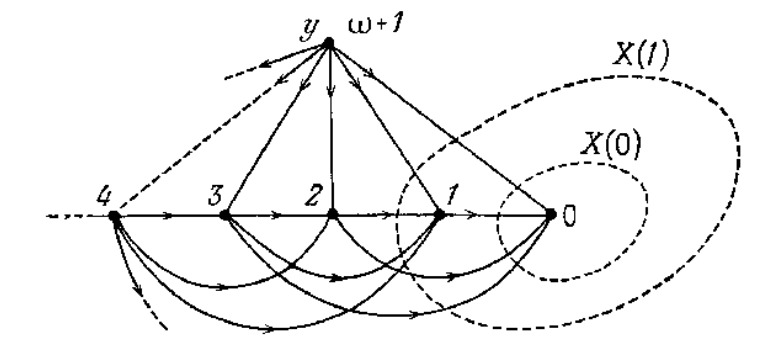
\includegraphics[width=0.5\textwidth]{graph.png}
\end{center}

\textbf{Рис. 3--2}

Пример. У графа, изображенного на рис. 3--2, каждая вершина $x$ имеет порядок $o(x)$, который указан на чертеже, лишь одна вершина $y$ имеет трансфинитный порядок. Здесь $X = X(\omega + 1)$.

\textbf{Теорема 4} Порядковая функция определена на всем множестве $X$ в том и только в том случае, если граф $(X, \Gamma)$ прогрессивно конечен.

1$^\circ$ Пусть $\theta(x)$ существует для всех $x \in X$, покажем, что граф прогрессивно конечен. С этой целью мы допустим, что существует бесконечный путь $[a_1, a_2, \ldots]$ и убедимся в том, что это приводит к противоречию.

Положим $A = \{a_1, a_2, \ldots\}$; имеем $A \cap X(\emptyset) = \emptyset$. Если $A \cap X(\beta) = \emptyset$ для всех порядковых чисел $\beta < \alpha$, то также $A \cap X(\alpha) = \emptyset$. Тогда в силу принципа индукции, $A \cap X = \emptyset$.

Отсюда $A = \emptyset$, что невозможно.

2$^\circ$ Наоборот, предположим, что существует вершина $x$, не имеющая порядка, пусть $B$ — множество всех таких вершин. Имеем $B \neq \emptyset$.

Если $x_1 \in B \cap \Gamma^*(x)$ (либо $x_1 \notin X(0)$) поэтому в $X_1$ найдется вершина $x_2 \in B$, точно так же в $\Gamma_{x_2}$ найдется вершина $x_3 \in B$ и т.д.

Путь $[x_1, x_2, x_3, \ldots]$ обладает бесконечной длиной, и граф не может быть прогрессивно конечным.
c